% Partial sums of 1-1+1-1 and their running averages.
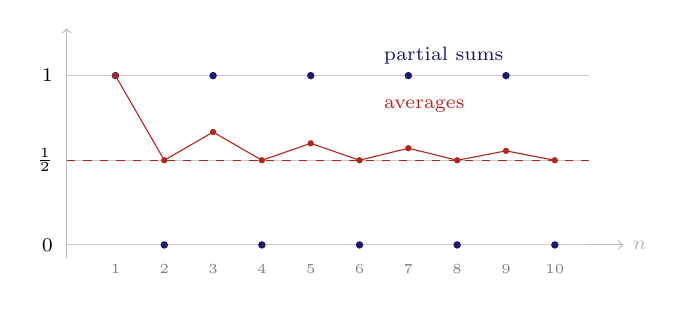
\begin{tikzpicture}[x=0.62cm,y=2.15cm]
  \draw[gray!55,->] (0,0) -- (11.4,0) node[right,font=\scriptsize] {$n$};
  \draw[gray!55,->] (0,-0.08) -- (0,1.28);
  \foreach \y/\lab in {0/0,0.5/\frac12,1/1} {
    \draw[gray!40] (0,\y) -- (10.7,\y);
    \node[font=\scriptsize,anchor=east] at (-0.08,\y) {$\lab$};
  }
  \draw[BrickRed,dashed] (0,0.5) -- (10.7,0.5);
  % partial sums: 1,0,1,0,...
  \foreach \n in {1,3,5,7,9} {\fill[MidnightBlue] (\n,1) circle (1.35pt);}
  \foreach \n in {2,4,6,8,10} {\fill[MidnightBlue] (\n,0) circle (1.35pt);}
  % averages: 1, 1/2, 2/3, 1/2, 3/5, 1/2, 4/7, 1/2, 5/9, 1/2
  \fill[BrickRed] (1,1) circle (1.15pt);
  \fill[BrickRed] (2,0.5) circle (1.15pt);
  \fill[BrickRed] (3,0.6667) circle (1.15pt);
  \fill[BrickRed] (4,0.5) circle (1.15pt);
  \fill[BrickRed] (5,0.6) circle (1.15pt);
  \fill[BrickRed] (6,0.5) circle (1.15pt);
  \fill[BrickRed] (7,0.5714) circle (1.15pt);
  \fill[BrickRed] (8,0.5) circle (1.15pt);
  \fill[BrickRed] (9,0.5556) circle (1.15pt);
  \fill[BrickRed] (10,0.5) circle (1.15pt);
  \draw[BrickRed,thin] plot coordinates {(1,1) (2,0.5) (3,0.6667) (4,0.5) (5,0.6) (6,0.5) (7,0.5714) (8,0.5) (9,0.5556) (10,0.5)};
  \node[font=\scriptsize,MidnightBlue,anchor=west] at (6.3,1.12) {partial sums};
  \node[font=\scriptsize,BrickRed,anchor=west] at (6.3,0.82) {averages};
  \foreach \n in {1,2,3,4,5,6,7,8,9,10} {
    \node[font=\tiny,gray,anchor=north] at (\n,-0.06) {$\n$};
  }
\end{tikzpicture}
